\documentclass{article}
\usepackage[utf8]{inputenc}
\usepackage[margin=1in]{geometry}
\usepackage{amsmath}
\usepackage{amssymb}
\usepackage{braket} % For Dirac notation < | >
\usepackage{fancyhdr}
\usepackage{enumitem}
\usepackage{tikz}
\usepackage{}
% Setup for headers and footers
\pagestyle{fancy}
\fancyhf{} % Clear all headers and footers
\fancyhead[L]{Electrodynamics}
\fancyhead[C]{(Chapter 3)}
\fancyhead[R]{Worksheet PS.10}
\fancyfoot[C]{\thepage}
\renewcommand{\headrulewidth}{0.4pt}
% Title block for the first page
\fancypagestyle{plain}{
    \fancyhf{}
    \fancyfoot[C]{\thepage}
    \renewcommand{\headrulewidth}{0pt}
}
\begin{document}
\thispagestyle{plain}

\begin{center}
    {\Large Electrodynamics}\\
    {\Large Worksheet PS.10}\\
    \vspace{0.2cm}
    (Chapter 3)\\
    December 8, 2025\\
    Zoeb Izzi
\end{center}

\vspace{0.5cm}

% Problem 1
\noindent \textbf{1. Applying quantum ideas to kinematics}
\hrule
\vspace{0.3cm}

\noindent Suppose someone drops a rock off a cliff of height $h$. As it falls, you decide to snap a million pictures at random intervals. In each image, you measure the distance the rock has fallen.

\begin{enumerate}[label=\alph*.]
    \item What is the position of the rock as a function of time? Use your AP Physics skills and only employ \textit{classical} kinematics. For a reference frame, set the ground as $ y = 0$ and upward as the positive $y$ direction. 
    \newline \newline 
    Trivially, we know that it is $\boxed{y = h - \frac{1}{2} g t^2}$. 
    \newline 
    \item What is the velocity of the rock as a function of time? Once again, \textit{only} use classical kinematics for this calculation.
    \newline \newline 
    Once again, we trivially deduce that $\boxed{v = -gt}$.
    \newline
    \item What is the total time the rock is in the air?
    \newline
    \[0 = h - \frac 1 2 gt^2, \boxed{t = \sqrt{\frac{2h}{g}}}\]
    \item Determine an expression for the probability density in terms of height ($y$) for the ball as it falls.
    \\ 
    \[t = \sqrt{\frac{2(h-y)}{g}}
        \implies
        \left|\frac{\mathrm{d}t}{\mathrm{d}y}\right| = \frac{1}{\sqrt{2g(h-y)}} \implies \boxed{\rho(y) = \frac{1}{2\sqrt{h(h-y)}}, \quad 0 \le y \le h}\]
    \item Confirm that your probability density correctly predicts that the rock MUST be found somewhere between $ y = 0$ and $y=h$. 
    \\ 
    \[
        \int_0^h \rho(y)\,\mathrm{d}y
        = \frac{1}{2\sqrt{h}}\int_0^h (h-y)^{-1/2}\,\mathrm{d}y
        = \frac{1}{2\sqrt{h}}\Big[-2\sqrt{h-y}\Big]_0^h
        = \frac{1}{2\sqrt{h}}\cdot 2\sqrt{h} = 1 \checkmark
    \]
    Since the probability that it lies in this interval is 1, it must be the case that the probability it lies outside this interval is $1-1 = 0$, so it cannot lie outside the specified interval.
    \item Use your probability density to calculate the expectation value of the position of the ball over the course of its entire flight. Why is this expectation value greater than $\frac h 2$?
    \\
    \[
        \langle y \rangle
        = \int_0^h y\,\rho(y)\,\mathrm{d}y
        = \frac{1}{2\sqrt{h}}\int_0^h \frac{y}{\sqrt{h-y}}\,\mathrm{d}y= \frac{1}{2\sqrt{h}}\int_0^h \frac{h-u}{\sqrt{u}}\,\mathrm{d}u
        = \frac{1}{2\sqrt{h}}\left[h \cdot 2\sqrt{h} - \frac{2}{3}h^{3/2}\right]
        = \frac{1}{2\sqrt{h}}\cdot\frac{4}{3}h^{3/2}
        = \boxed{\frac{2h}{3}}
    \]
    It makes sense that this value is greater than $\frac h 2$ since we have an acceleration, which means it moves faster (thereby spending less time) when closer to the ground, so it would spend a larger percentage of it's time slightly higher - in this case, $33\%$ higher. 
\end{enumerate}

\vspace{0.5cm}


\noindent \textbf{2. Normalizing a wavefunction in the position basis}
\hrule
\vspace{0.3cm}

A particle is represented by the wave function:
\[\phi(x) =  \begin{cases} 
      A(x/a) & 0 \leq x \leq a \\
      A(b-x)/(b-a) & a\leq x \leq b \\
      0 & otherwise 
   \end{cases}\]
 \[  \text{Where $A, a, $ and $ b$ are positive constants.}\]

 \begin{enumerate}[label=\alph*.]
    \item Normalize $\phi(x)$ (i.e. find $A$ in terms of $a$ and $b$.)
    \\
    \[
        \int_0^a A^2\!\left(\frac{x}{a}\right)^{\!2}\mathrm{d}x
        = \frac{A^2}{a^2}\cdot\frac{a^3}{3} = \frac{A^2 a}{3}\\[4pt]
        \]\[\int_a^b A^2\frac{(b-x)^2}{(b-a)^2}\,\mathrm{d}x
        = \frac{A^2}{(b-a)^2}\cdot\frac{(b-a)^3}{3} = \frac{A^2(b-a)}{3}
    \]\[(1) + (2) = \frac{A^2b}{3} = 1 \implies \boxed{A = \sqrt{\frac{3}{b}}}\]
    \item Sketch $\phi(x)$ as a function of $x$.
    \\
    \begin{center}
    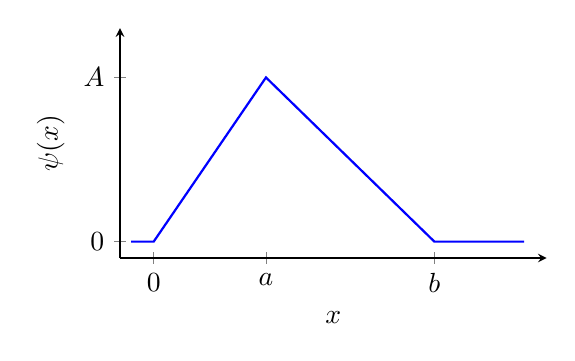
\begin{tikzpicture}
        \begin{axis}[
            width=7cm, height=4.5cm,
            xmin=-0.3, xmax=3.5,
            ymin=-0.1, ymax=1.3,
            xlabel={$x$}, ylabel={$\psi(x)$},
            xtick={0,1,2.5},
            xticklabels={$0$,$a$,$b$},
            ytick={0,1},
            yticklabels={$0$,$A$},
            axis lines=left,
            clip=false,
        ]
        \addplot[thick, blue] coordinates {(-0.2,0)(0,0)(1,1)(2.5,0)(3.3,0)};
        \end{axis}
    \end{tikzpicture}
    \end{center}
    \item Where is the particle most likely to be found?
    \\ \\ 
    Trivially, from the graph, at $x = a$.
    \item What is the probability of finding the particle to the left of $a$? Check your result in the limiting cases, $b = a, 2a$.
    \item If many measurements of the position ($x$) of this particle were made, what would be the average location the particle was found in?
 \end{enumerate}



\vspace{0.5cm}

% Problem 3
\noindent \textbf{3. Expectation Values \& Uncertainty}
\hrule
\vspace{0.3cm}

\noindent A particle is represented (at time $t=0$) by the wave function:
\[\phi(x) =  \begin{cases} 
      A(a^2-x^2) & -a\leq x \leq a \\
      0 & otherwise 
   \end{cases}\]

\begin{enumerate}[label=\alph*.]
    \item Determine the normalization constant $A$.
    \item What is the expectation value of $x$?
    \item What is the expectation value of $p$?
    \item Find the expectation value of $x^2$.
    \item Find the expectation value of $p^2$.
    \item Find the uncertainty in $x$ ($\sigma_x$).
    \item Find the uncertainty in $p$ ($\sigma_p$).
    \item Check that your results are consistent with the uncertainty principle.
\end{enumerate}

\noindent \textbf{4. Infinite Square Well}
\hrule
\vspace{0.3cm}

\noindent A particle in the infinite square well has the initial wave function $\psi(x) = Ax(a-x)$ for $(0 \leq x \leq a)$. Outside of this domain, the wave function is, of course, $\psi(x) = 0$.
\begin{enumerate}[label=\alph*.]
    \item Find the normalization constant $A$.
    \item We know we can always decompose any initial state into a superposition of eigenstates. We can write out this superposition as:
    \[\psi(x) = \sum_{n=1} c_n\phi(n)\]
    where we can determine the expansion coefficients using the overlap integral:
    \[c_n = \int_{0}^{a} \phi(x) \cdot \psi(x)dx\]
    with the eigenfunctions
    \[\phi_n = \sqrt{\frac 2 a} \sin\left(\frac{n\pi}{a}x\right)\]
    Determine expressions for the values of $c_n$ for $n=$ even integers and odd integers.
    \item Make a plot (using Python, Desmos, etc) of $\psi(x)$ (as initially defined) and your expansion for $\displaystyle \psi(x) = \sum_{n=1}c_n\phi_n$. Let $a=1$, and use only $n=1,2,3$. How well do these two functions match?
    \item What is the probability that the wave function $\psi(s)$ gets measured to be in the ground state $n=1$?
\end{enumerate}

\end{document}